%Fiquemos com Deus e Nossa Senhora!
%Sao Jose de Cupertino rogai por nos!!
%Honra teu pai e tua mae!
% ### Uses XeLaTeX ### %
% ### Needs beamer-master ### %
\documentclass[aspectratio=169]{beamer} %. Aspect Ratio 16:9

\usetheme{AI2} % beamerthemeSprace.sty
\usepackage[portuguese]{babel}
\usepackage[utf8]{inputenc}
\usepackage[T1]{fontenc}
\usepackage{ragged2e,bm}

\DeclareMathOperator*{\argmin}{arg\,min}
\DeclareMathOperator*{\argmax}{arg\,max}

% DATA FOR FOOTER
\date{2025}
\title{- Análise de Algoritmos}
\author{João Paulo Papa}
\institute{Análise de Algoritmos}

\begin{document}
% ####################################
% FIRST SLIDE 						:: \SliTit{This is the Title of the Talk}{A. B. Name}{Sprace}
% SUB-TITLE SLIDE 					:: \SliSubTit{<title>}{<explanation}
% SUB-SUB-TITLE SLIDE				:: \SliSubSubTit{<title>}{<explanation}
% SLIDE WITH TITLE 					:: \SliT{Title}{Content}
% SLIDE NO TITLE 						:: \Sli{Content} 
% SLIDE DOUBLE COLUMN WITH TITLE 	:: \SliDT{Title}{First Column}{Second Column}
% SLIDE DOUBLE COLUMN NO TITLE 		:: \SliD{First Column}{Second Column}
% SLIDE ADVANCED WITH TITLE 			:: \SliAdvT{Title}{Content}
% SLIDE ADVANCED NO TITLE 			:: \SliAdv{Content}
% SLIDE ADVANCED DOUBLE WITH TITLE 	:: \SliAdvDT{Title}{First Column}{Second Column}
% SLIDE ADVANCED DOUBLE NO TITLE 	:: \SliAdvD{First Column}{Second Column}
% SLIDE BLACK						:: \Black{ <Content> }
% SLIDE WHITE						:: \White{ <Content> }
% ITEMIZATION 						:: \begin{itemize}  \iOn{First} \iTw {Second} \iTh{Third} \end{itemize}
% COMMENT TEXT				 		:: \note{<comment>}
% SECTION 							:: \secx{Section} | \secxx{Sub-Section}
% BOLD SPRACE COLOR				:: \bfs{<text>}
% TABLE OF CONTENT					:: \tocitem{<title>}{<content>}
% LEFT ALIGN EQUATION				:: \begin{flalign*}  & <equation> &   \end{flalign*}
% CENTER ALIGN EQUATION	S			:: \begin{gather*} <equations>  \end{gather*}
% SLASH								:: \slashed{<>}
% BAR								:: \barr{<letter>} instead of \bar{<letter>}
% THEREFORE						:: use \portanto (larger and bold}
% 2 or 3 MATH SYMBOLS				:: \overset{<up>}{<down>} &  \underset{<below>}{\overset{<above>}{<middle>}}  
% INSERT TEXT IN FORMULA			:: \ins{<text>}
% EXERCISE							:: \exe{<exercise #>}{<exercise text>}
% SUGGESTED READING BOX			:: \sug{<references>}
% CITATION							:: \cittex{<citation>}
% CITATION DOUBLE COLUMN 			:: \cittexD{<citation>}
% TEXT POSITION						:: \texpos{<Xcm>}{<Ycm>}{<text>} origin = center of slide : x right | y down
% REFERENCE AT BOTTOM  S/D SLIDE		:: \refbotS{<reference>} \refbotD{<reference>}
% HIDDEN SLIDE						:: \hid
% COLOR BOX 						:: \blu{blue} + \red{rec} + \yel{yellow} + \gre{green} + \bege{beige}
% FRAME 							:: \fra{sprace} \frab{blue} \frar{red} + \fray{yellow} + \frag{green}		
% FIGURE 							:: \img{X}{Y}{<scale>}{Figure.png} 
% FIGURE							:: \includegraphics[scale=<scale>]{Figures/.png}
% FIGURE DOUBLE SLIDE NO TITLE		::  \img{-4}{0.5}{<scale>}{Figure.png} % Image 1st half
%									::  \img{4}{0.5}{<scale>}{Figure.png} % Image 2nd half
% FIGURE DOUBLE SLIDE WITH TITLE		::  \img{-4}{0}{<scale>}{Figure.png} % Image 1st half
%									::  \img{4}{0}{<scale>}{Figure.png} % Image 2nd half
% INCLUDING SWF (Flash)				:: \usepackage{media9} and \includemedia >> USE ACROBAT <<
%%%%%%%%%%%%%%%%%%%%%%%%%%%%%%%%%%%%%%%%%%%%%%%%%%
% ###############################################################################
% FIRST SLIDE
\SliTit{Aula 1 - Crescimento de Funções}{Análise de Algoritmos}{}{João Paulo Papa (UNESP/Bauru)}
%%%%%%%%%%%%%%%%%%%%%%%%%%%%%%%%%%%%%%%%%%%%%%%%%%
% ###############################################################################
% SLIDE SUB-TITLE
%\SliSubTit{Sub-Title}{Description}{}
%%%%%%%%%%%%%%%%%%%%%%%%%%%%%%%%%%%%%%%%%%%%%%%%%%
% ###############################################################################
%\SliSubSubTit{Sub-Sub-Title}{Description}
 %%%%%%%%%%%%%%%%%%%%%%%%%%%%%%%%%%%%%%%%%%%%%%%%%%



\SliT{Introdução}{
\justifying Nesta aula iremos abordar os seguintes assuntos:

\begin{itemize}
	\item Objetivo da disciplina.
	\item Notação de Landau.
	\item Crescimento assintótico de funções.
\end{itemize}
}

\SliT{Objetivo da Disciplina}{
\justify O objetivo da disciplina é oferecer o \textbf{ferramental matemático} para que possamos \textbf{analisar} um algoritmo e estimar a sua \textbf{complexidade}.

\justify Qual o objetivo desta análise? Com ela, podemos, por exemplo, \textbf{comparar} diferentes propostas de solução para um determinado problema de maneira \textbf{agnóstica} a:

\begin{itemize}
	\item Sistema operacional.
	\item Compilador.
	\item Linguagem de programação.
	\item Arquitetura do computador.
\end{itemize}
}

\SliT{Notação de Landau}{
\justify O alemão \textbf{Edmund Landau} inventou símbolos que são utilizados na área da Ciência da Computação e Matemática para descrever o \textbf{comportamento assintótico} de funções. Basicamente, este simbolismo nos diz quão rápida uma função \textbf{cresce} ou \textbf{decresce}. Basicamente, temos cinco símbolos:

\begin{itemize}
	\item $O$: descreve o limite \textbf{estritamente superior} de uma função (conhecido como \emph{Big O}).
	\item $\Theta$: descreve o limite \textbf{médio} de uma função.
	\item $o$: descreve o limite \textbf{superior} de uma função.
	\item $w$: descreve o limite \textbf{inferior} de uma função.
	\item $\Omega$: descreve o limite \textbf{estritamente inferior} de uma função.
\end{itemize}
}

\SliT{Crescimento Assintótico de Funções}{

\justify Vejamos o gráfico a seguir. Ele representa a seguinte relação quando $n\rightarrow\infty$:

\begin{equation}
1 <\log(n)<n<n\log(n)<n^2<2.5^n.
\end{equation}

\begin{center}
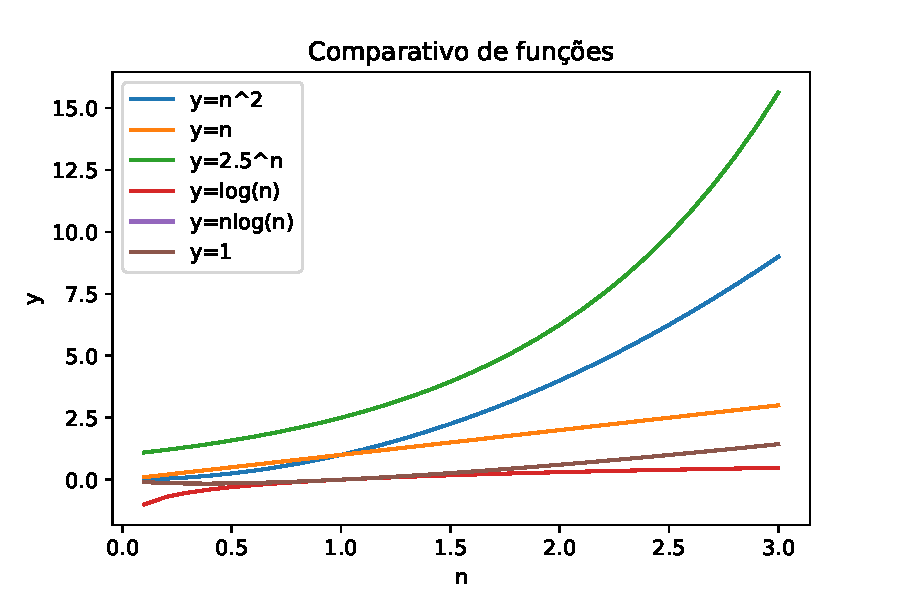
\includegraphics[scale=0.47]{./src/funcoes.pdf}\hspace{1cm}
\end{center}
}

\Sli{
No entanto, podemos generalizar a Equação 1 da seguinte forma:

\begin{equation}
\label{e.crescimento_assintotico_generalizado}
1 <\log(n)<\sqrt{n}<n<n\log(n)<n^2<n^3<\ldots<2^n<2.5^n<3^n<\ldots<n^n.
\end{equation}

\justify Qual a definição de $O(n)?$ 

\setbeamercolor{BoxColour}{fg=black,bg=gray!30}
\begin{beamercolorbox}[sep=1em,wd=13.4cm]{BoxColour}
   Uma função $f(n)\in O(g(n))$ sse $\exists c,n_o\in\mathbb{R}^+$ tal que $f(n)\leq cg(n)$, $\forall n\geq n_0$.
\end{beamercolorbox}\medskip

\justify \underline{Exemplo:} sejam as funções $f(n)=2n+3$ e $g(n)=n$. Assumindo que $c=10$ e $n_0=1$, temos que $f(n)\leq 10g(n)\implies2n+3\leq 10n$, $n\geq 1$. Assim sendo, temos que $f(n)\in O(g(n)$, ou seja, que $2n+3\in O(n)$. \textbf{Na prática, existem diversos valores para $c$ que satisfazem a relação $\bm{f(n)\in O(g(n))}$}.
}

\Sli{
\justify Vamos para um segundo exemplo. Continuemos assumindo que $f(n)=2n+3$, mas agora temos que $g(n)=n^2$. Pergunta: $f(n)\in O(g(n))$?

\justify Novamente, basta encontrarmos valores para $c$ e $n_0$ que satisfaçam a nossa definição anterior. Um exemplo seria $c=5$ e $n_0= 1$. Neste caso, teremos que $f(n)\leq 5g(n)\implies2n+3\leq5n^2$, $n \geq 1$. Novamente, temos que $f(n)\in O(g(n)$, ou seja, que $2n+3\in O(n^2)$. 

\justify Podemos continuar com outros exemplos e veremos que $2n+3\in O(n^3)$, e assim por diante. Assim, podemos estabelecer uma definição para \textbf{informal} para a notação $O$.

\begin{equation*}
1 <\log(n)<\sqrt{n}<\overbrace{n<n\log(n)<n^2<n^3<\ldots<2^n<2.5^n<3^n<\ldots<n^n}^{\in O(n)}.
\end{equation*}
}

\end{document}